\subsection{WideResNet-22 on CIFAR-10}\label{cifar-10-results}

\begin{table}[t]
    \captionsetup{aboveskip=\tableaboveskip,belowskip=\tablebelowskip}
    \caption{\textbf{WideResNet-22-2 on CIFAR10}, tabulated for two density $(1-s)$ values. We group methods by their FLOP requirement and in each group, we mark the best accuracy in bold. Similar to \citet{rigl}, we assume that algorithms utilize sparsity during training. All results are obtained by methods implemented in our unified codebase.}
    \label{tab:cifar10-main-results}
    \centering
    
    \begin{tabular}{ c cc cc }
    \toprule
    \multirow{3}{*}{\textbf{Method}}& 
    \multicolumn{2}{c}{$\mathbf{1 - s=0.1}$} & \multicolumn{2}{c}{$\mathbf{1 - s=0.2}$} \\
    \cmidrule(lr){2-3} \cmidrule(lr){4-5}
    {} & 
    \makecell{Accuracy $\uparrow$ \\ (Test)}  & \makecell{FLOPs $\downarrow$  \\ (Train, Test)} &
    \makecell{Accuracy $\uparrow$ \\ (Test)}  & \makecell{FLOPs $\downarrow$  \\ (Train, Test)} \\
    \midrule
    Small Dense & 
    {89.0 $\pm$ 0.35} & {0.11x, 0.11x} & 
    {91.0 $\pm$ 0.07} & {0.20x, 0.20x} \\
    
    Static & 
    {89.1 $\pm$ 0.17} & {0.10x, 0.10x} & 
    {91.2 $\pm$ 0.16} & {0.20x,0.20x} \\

    SET &
    {91.3 $\pm$ 0.47} & {0.10x, 0.10x} & 
    \textbf{92.7 $\pm$ 0.28} & {0.20x, 0.20x} \\
    
    \textbf{RigL} &
    \textbf{91.7 $\pm$ 0.18} & {0.10x, 0.10x} &
    {92.6 $\pm$ 0.10} & {0.20x, 0.20x} \\
    \midrule
    
    SET (ERK)&
    {92.2 $\pm$ 0.04} & {0.17x, 0.17x} &
    {92.9 $\pm$ 0.16} & {0.35x, 0.35x} \\
    
    \textbf{RigL (ERK)} &
    \textbf{92.4 $\pm$ 0.06} & {0.17x, 0.17x} &
    \textbf{93.1 $\pm$ 0.09} & {0.35x, 0.35x} \\
    \midrule
    {Static\textsubscript{$2 \times$}} &
    {89.15 $\pm$ 0.17} & {0.20x, 0.10x} &
    {91.2 $\pm$ 0.16} & {0.40x, 0.20x} \\
    
    Lottery & 
    {90.4 $\pm$ 0.09} & {0.45x, 0.13x} & 
    {92.0 $\pm$ 0.31} & {0.68x,0.27x} \\
    
    {SET\textsubscript{$2 \times$}} &
    {83.3 $\pm$ 15.33} & {0.20x, 0.10x} &
    {93.0 $\pm$ 0.22} & {0.41x, 0.20x} \\
    
    SNFS & 
    {92.4 $\pm$ 0.43} & {0.51x, 0.27x} & 
    {92.7 $\pm$ 0.20} & {0.66x, 0.49x} \\ 
    
    SNFS (ERK)& 
    {92.2 $\pm$ 0.2} & {0.52x, 0.28x} & 
    {92.8 $\pm$ 0.07} & {0.66x, 0.49x} \\
    
    {SNFS\textsubscript{$2 \times$}} &
    {92.3 $\pm$ 0.33} & {1.02x, 0.27x} &
    {93.2 $\pm$ 0.14} & {1.32x, 0.98x} \\
    
    {RigL\textsubscript{$2 \times$}} &
    {92.3 $\pm$ 0.25} & {0.20x, 0.10x} &
    {93.0 $\pm$ 0.21} & {0.41x, 0.20x} \\
    
    % {RigL\textsubscript{$3 \times$}} &
    % {92.5 $\pm$ 0.11} & {0.30x, 0.10x} &
    % {93.2 $\pm$ 0.20} & {0.61x, 0.20x} \\
    
    {Pruning} & 
    {92.6 $\pm$ 0.08} & {0.32x,0.13x} & 
    {93.2 $\pm$ 0.27} & {0.41x,0.27x} \\ 
    
    \textbf{RigL\textsubscript{$2 \times$} (ERK)} &
    \textbf{92.7 $\pm$ 0.37} & {0.34x, 0.17x} &
    \textbf{93.3 $\pm$ 0.09} & {0.70x, 0.35x} \\
    \midrule
    
    \textbf{Dense Baseline} &
    \textbf{93.4 $\pm$ 0.07} & {9.45e8, 3.15e8} &
    \textbf{-} & {-} \\
    \bottomrule
    
    \end{tabular}
\end{table}
   
Results on the CIFAR-10 dataset are provided in Table \ref{tab:cifar10-main-results}. Tabulated metrics are averaged across 3 random seeds and reported with their standard deviation. All sparse networks use random initialization, unless indicated otherwise.\\

While SET improves over the performance of static sparse networks and small-dense networks, methods utilizing gradient information (SNFS, \textit{RigL}) obtain better test accuracies. SNFS can outperform \textit{RigL}, but requires a much larger training budget, since it (a) requires dense gradients at each training step, (b) redistributes layer-wise sparsity during mask updates. For all sparse methods, excluding SNFS, using ERK initialization improves performance, but with increased FLOP consumption. We calculate theoretical FLOP requirements in a manner similar to \citet{rigl} (exact procedure is described in the appendix). \\

Figure \ref{fig:cifar10-main-results} contains test accuracies of select methods across two additional sparsity values: ($0.5, 0.95$). At lower sparsities (higher densities), \textit{RigL} matches the performance of the dense baseline. Performance further improves by training for longer durations. Particularly, training \textit{RigL} (ERK) twice as long at 90\% sparsity exceeds the performance of iterative pruning while requiring similar theoretical FLOPs. This validates the original authors' claim that \textit{RigL} (a sparse-to-sparse training method) outperforms pruning (a dense-to-sparse training method). 

\begin{figure}[!t]
    \centering
    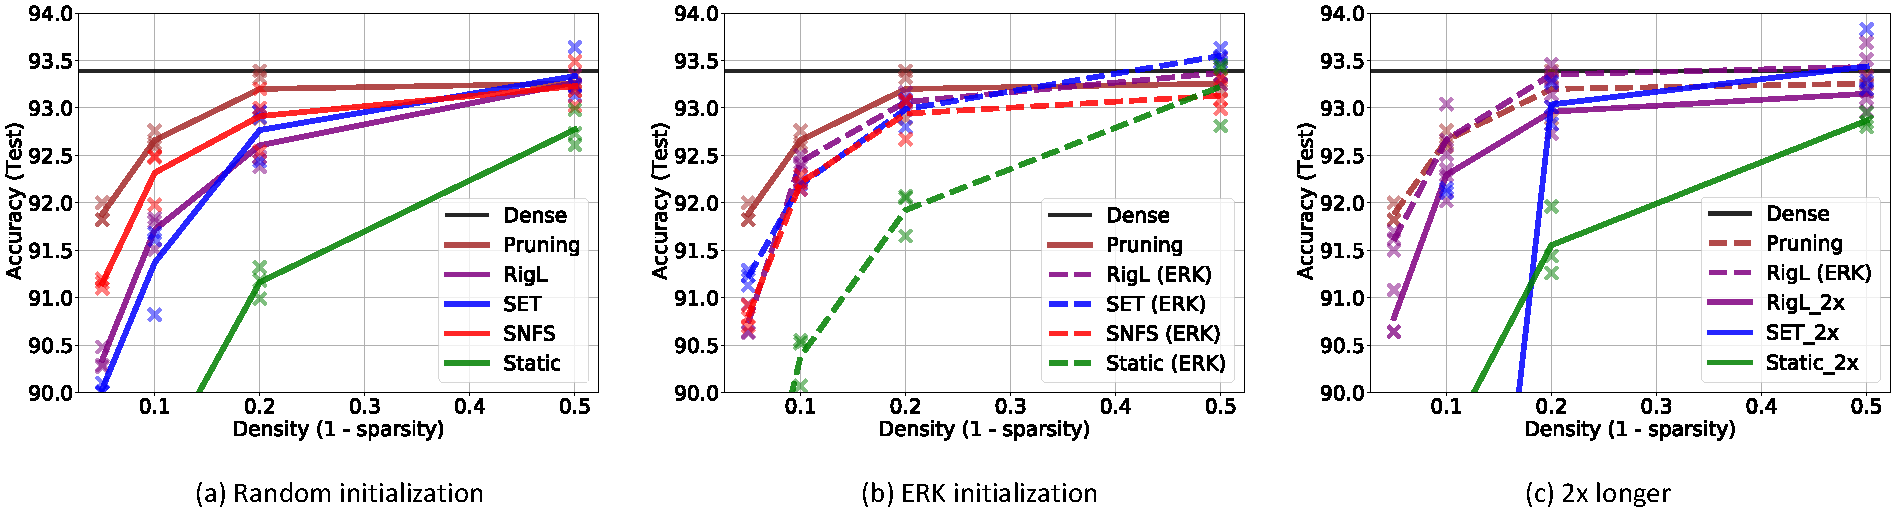
\includegraphics[width=1\textwidth]{../openreview/figs/cifar10_main.pdf}
    \captionsetup{aboveskip=\figureaboveskip,belowskip=\figurebelowskip}
    \caption{\textbf{Test Accuracy vs Sparsity on CIFAR-10,} plotted for Random initialization \textbf{(left)}, ERK initialization \textbf{(center)}, and for training $2\times$ longer \textbf{(right)}. Owing to random growth, SET can be unstable when training for longer durations with higher sparsities. Overall, \textit{RigL}\textsubscript{$2 \times$} (ERK) achieves highest test accuracy.}
    \label{fig:cifar10-main-results}
\end{figure}